%%%%%%%%%%%%%%%%%%%%%%%%%%%%%%%%%%%%%%%%%
% Programming/Coding Assignment
% LaTeX Template
%
% This template has been downloaded from:
% http://www.latextemplates.com
%
% Original author:
% Ted Pavlic (http://www.tedpavlic.com)
%
% Note:
% The \lipsum[#] commands throughout this template generate dummy text
% to fill the template out. These commands should all be removed when 
% writing assignment content.
%
% This template uses a Perl script as an example snippet of code, most other
% languages are also usable. Configure them in the "CODE INCLUSION 
% CONFIGURATION" section.
%
%%%%%%%%%%%%%%%%%%%%%%%%%%%%%%%%%%%%%%%%%

%----------------------------------------------------------------------------------------
%	PACKAGES AND OTHER DOCUMENT CONFIGURATIONS
%----------------------------------------------------------------------------------------

\documentclass{article}
\usepackage{fancyhdr} % Required for custom headers
\usepackage{lastpage} % Required to determine the last page for the footer
\usepackage{extramarks} % Required for headers and footers
\usepackage[usenames,dvipsnames]{color} % Required for custom colors
\usepackage{graphicx} % Required to insert images
\usepackage{caption}
\usepackage{listings} % Required for insertion of code
\usepackage{courier} % Required for the courier font
\usepackage{lipsum} % Used for inserting dummy 'Lorem ipsum' text into the template
\usepackage[colorlinks=true,linkcolor=black,anchorcolor=black,citecolor=black,menucolor=black,runcolor=black,urlcolor=black,bookmarks=true]{hyperref}
\usepackage[table,svgnames]{xcolor}
\usepackage{tabularx}
\usepackage{booktabs}
\usepackage{natbib}
\usepackage{hyperref}
\usepackage{natbib}
\usepackage{underscore}
\usepackage{subfigure}

% Margins
\topmargin=-0.45in
\evensidemargin=0in
\oddsidemargin=0in
\textwidth=6.5in
\textheight=9.0in
\headsep=0.25in

\linespread{1.1} % Line spacing

% Set up the header and footer
\pagestyle{fancy}
\lhead{\hmwkAuthorName} % Top left header
\chead{\hmwkClass\ (\hmwkClassInstructor\ \hmwkClassTime): \hmwkTitle} % Top center head
\rhead{\firstxmark} % Top right header
\lfoot{\lastxmark} % Bottom left footer
\cfoot{} % Bottom center footer
\rfoot{Page\ \thepage\ of\ \protect\pageref{LastPage}} % Bottom right footer
\renewcommand\headrulewidth{0.4pt} % Size of the header rule
\renewcommand\footrulewidth{0.4pt} % Size of the footer rule

\setlength\parindent{0pt} % Removes all indentation from paragraphs

%----------------------------------------------------------------------------------------
%	CODE INCLUSION CONFIGURATION
%----------------------------------------------------------------------------------------

\definecolor{MyDarkGreen}{rgb}{0.0,0.4,0.0} % This is the color used for comments
\lstloadlanguages{Perl} % Load Perl syntax for listings, for a list of other languages supported see: ftp://ftp.tex.ac.uk/tex-archive/macros/latex/contrib/listings/listings.pdf
\lstset{language=Perl, % Use Perl in this example
        frame=single, % Single frame around code
        basicstyle=\small\ttfamily, % Use small true type font
        keywordstyle=[1]\color{Blue}\bf, % Perl functions bold and blue
        keywordstyle=[2]\color{Purple}, % Perl function arguments purple
        keywordstyle=[3]\color{Blue}\underbar, % Custom functions underlined and blue
        identifierstyle=, % Nothing special about identifiers                                         
        commentstyle=\usefont{T1}{pcr}{m}{sl}\color{MyDarkGreen}\small, % Comments small dark green courier font
        stringstyle=\color{Purple}, % Strings are purple
        showstringspaces=false, % Don't put marks in string spaces
        tabsize=5, % 5 spaces per tab
        %
        % Put standard Perl functions not included in the default language here
        morekeywords={rand},
        %
        % Put Perl function parameters here
        morekeywords=[2]{on, off, interp},
        %
        % Put user defined functions here
        morekeywords=[3]{test},
       	%
        morecomment=[l][\color{Blue}]{...}, % Line continuation (...) like blue comment
        numbers=left, % Line numbers on left
        firstnumber=1, % Line numbers start with line 1
        numberstyle=\tiny\color{Blue}, % Line numbers are blue and small
        stepnumber=5 % Line numbers go in steps of 5
}

% Creates a new command to include a perl script, the first parameter is the filename of the script (without .pl), the second parameter is the caption




%----------------------------------------------------------------------------------------
%	DOCUMENT STRUCTURE COMMANDS
%	Skip this unless you know what you're doing
%----------------------------------------------------------------------------------------

% Header and footer for when a page split occurs within a problem environment
\newcommand{\enterProblemHeader}[1]{
\nobreak\extramarks{#1}{#1 continued on next page\ldots}\nobreak
\nobreak\extramarks{#1 (continued)}{#1 continued on next page\ldots}\nobreak
}

% Header and footer for when a page split occurs between problem environments
\newcommand{\exitProblemHeader}[1]{
\nobreak\extramarks{#1 (continued)}{#1 continued on next page\ldots}\nobreak
\nobreak\extramarks{#1}{}\nobreak
}

\setcounter{secnumdepth}{0} % Removes default section numbers
\newcounter{homeworkProblemCounter} % Creates a counter to keep track of the number of problems

\newcommand{\homeworkProblemName}{}
\newenvironment{homeworkProblem}[1][Problem \arabic{homeworkProblemCounter}]{ % Makes a new environment called homeworkProblem which takes 1 argument (custom name) but the default is "Problem #"
\stepcounter{homeworkProblemCounter} % Increase counter for number of problems
\renewcommand{\homeworkProblemName}{#1} % Assign \homeworkProblemName the name of the problem
\section{\homeworkProblemName} % Make a section in the document with the custom problem count
\enterProblemHeader{\homeworkProblemName} % Header and footer within the environment
}{
\exitProblemHeader{\homeworkProblemName} % Header and footer after the environment
}

\newcommand{\problemAnswer}[1]{ % Defines the problem answer command with the content as the only argument
\noindent\framebox[\columnwidth][c]{\begin{minipage}{0.98\columnwidth}#1\end{minipage}} % Makes the box around the problem answer and puts the content inside
}

\newcommand{\homeworkSectionName}{}
\newenvironment{homeworkSection}[1]{ % New environment for sections within homework problems, takes 1 argument - the name of the section
\renewcommand{\homeworkSectionName}{#1} % Assign \homeworkSectionName to the name of the section from the environment argument
\subsection{\homeworkSectionName} % Make a subsection with the custom name of the subsection
\enterProblemHeader{\homeworkProblemName\ [\homeworkSectionName]} % Header and footer within the environment
}{
\enterProblemHeader{\homeworkProblemName} % Header and footer after the environment
}

%----------------------------------------------------------------------------------------
%	NAME AND CLASS SECTION
%----------------------------------------------------------------------------------------

\newcommand{\hmwkTitle}{A8} % Assignment title
\newcommand{\hmwkDueDate}{Thursday,\ April\ 13,\ 2017} % Due date
\newcommand{\hmwkClass}{\ INTRO. TO WEB SCIENCE:\ CS 532} % Course/class
\newcommand{\hmwkClassTime}{} % Class/lecture time
\newcommand{\hmwkClassInstructor}{Dr. Nelson} % Teacher/lecturer
\newcommand{\hmwkAuthorName}{Udochukwu Nweke} % Your name

%----------------------------------------------------------------------------------------
%	TITLE PAGE
%----------------------------------------------------------------------------------------

\title{
\vspace{2in}
\textmd{\textbf{\hmwkClass:\ \hmwkTitle}}\\
\normalsize\vspace{0.1in}\small{Due\ on\ \hmwkDueDate}\\
\vspace{0.1in}\large{\textit{\hmwkClassInstructor\ \hmwkClassTime}}
\vspace{3in}
}

\author{\textbf{\hmwkAuthorName}}
\date{} % Insert date here if you want it to appear below your name

%----------------------------------------------------------------------------------------

\begin{document}

\maketitle

%----------------------------------------------------------------------------------------
%	TABLE OF CONTENTS
%----------------------------------------------------------------------------------------

%\setcounter{tocdepth}{1} % Uncomment this line if you don't want subsections listed in the ToC

\newpage
\tableofcontents
\newpage

%----------------------------------------------------------------------------------------
%	PROBLEM 1
%----------------------------------------------------------------------------------------

% To have just one problem per page, simply put a \clearpage after each problem

\begin{homeworkProblem}

\lstinputlisting[caption=Grab 100 Unique Blog Code, language=python]{P1.py}

\lstinputlisting[caption=Generate Feed Vector Code, language=python]{mod-generatefeedvector.py}
Create a blog-term matrix.  Start by grabbing 100 blogs; include:\\

\url{http://f-measure.blogspot.com/}\\
\url{http://ws-dl.blogspot.com/}//

and grab 98 more as per the method shown in class.  Note that this
method randomly chooses blogs and each student will separately do
this process, so it is unlikely that these 98 blogs will be shared
among students.  In other words, no sharing of blog data.  Upload
to github your code for grabbing the blogs and provide a list of
blog URIs, both in the report and in github.\\

Use the blog title as the identifier for each blog (and row of the
matrix).  Use the terms from every item/title (RSS) or entry/title
(Atom) for the columns of the matrix.  The values are the frequency
of occurrence.  Essentially you are replicating the format of the
"blogdata.txt" file included with the PCI book code.  Limit the
number of terms to the most ``popular'' (i.e., frequent) 1000 terms,
this is *after* the criteria on p. 32 (slide 7) has been satisfied.
Remember that blogs are paginated.  

\textbf{Solution 1:}\\

1. In order to grab 98 more unique blogs, I continuously dereferenced  \url{http://blogtimenow.com/blogging/find-blogger-blog-id-post-id-unique-id-number/} to grab a new blog each time. I used \url{ http://blogtimenow.com/blogging/
find-blogger-blog-id-post-id-unique-id-number/} to discover how to find the blog IDs. This is seen in \textit{getBlogs()} in Listing 1. The 100 unique blog url is displayed in Table \ref{tab:Unique Blogs}\\

2. I used \textit{generateFeedVector()} in (PCI code,listing 2). I extracted all the pages for each blog through \textit{getPagesForBlog\_pre()} (Listing 2) I also included line 148-163 in listing 2 in order to limit the number of terms to the most ``popular'' 1000 terms.



\begin{table}[h!]
 \centering
 \caption{100 Unique Blogs}
  \label{tab:Unique Blogs}
    \begin{tabular}{ |l| l | }
     \hline
 S/N & URL\\
 \hline
 1&\url{http://f-measure.blogspot.com/}\\
 \hline
 2&\url{http://ws-dl.blogspot.com/}\\
 \hline
 3&\url{http://antonellagiugliano.blogspot.com/}\\
 \hline
 4&\url{http://markeortega.blogspot.com/}\\
 \hline
 5&\url{http://myopiamuse.blogspot.com/}\\
 \hline
 6&\url{http://floorshimezipperboots.blogspot.com/}\\
 \hline
 7&\url{http://ps-music.blogspot.com/}\\
 \hline
 8&\url{https://chemical-robert.blogspot.com/}\\
 \hline
 9&\url{http://onestunningsingleegg.blogspot.com/}\\
 \hline
 10&\url{http://www.thestarkonline.com/}\\
 \hline
 11&\url{http://macthemost.blogspot.com/}\\
 \hline
 12&\url{http://psychfolkmusic.blogspot.com/}\\
 \hline
 13&\url{http://adrianomarquesblog.blogspot.com/}\\
 \hline
 14&\url{http://www.punkrockteaching.org/}\\
 \hline
 15&\url{http://cherryarea.blogspot.com/}\\
 \hline
 16&\url{http://doyouneedatv.blogspot.com/}\\
 \hline
 17&\url{http://ohyesjonsi.blogspot.com/}\\
 \hline
 18&\url{http://mts-dailythemes.blogspot.com/}\\
 \hline
 19&\url{http://www.thejeopardyofcontentment.com/}\\
 \hline
 20&\url{http://www.sonology.com/}\\
 \hline
 21&\url{http://jamiemclelland.blogspot.com/}\\
 \hline
 22&\url{http://organmyth.blogspot.com/}\\
 \hline
 23&\url{http://jbreitling.blogspot.com/}\\
 \hline
 24&\url{http://nonsensealamode.blogspot.com/}\\
 \hline
 25&\url{http://mondaywakeup.blogspot.com/}\\
 \hline
 26&\url{http://chantellesmedia2.blogspot.com/}\\
 \hline
 27&\url{http://doginasweatershowreviews.blogspot.com/}\\
 \hline
 28&\url{http://jojobethkatiehannahlcm1516.blogspot.com/}\\
 \hline
 29&\url{http://angie-dynamo.blogspot.com/}\\
 \hline
 30&\url{http://mandolinnn.blogspot.com/}\\
 \hline
 31&\url{http://ngaio1619.blogspot.com/}\\
 \hline
 32&\url{http://isyelili.blogspot.com/}\\
 \hline
 33&\url{http://earenjoy.blogspot.com/}\\
 \hline
 34&\url{http://tuqueresveristo.blogspot.com/}\\
 \hline
 35&\url{http://mediastudiesa2advanced.blogspot.com/}\\
 \hline
 36&\url{https://norecordshopsleft.blogspot.com/}\\
 \hline
 37&\url{http://bonjourgirl.blogspot.com/}\\
 \hline
 38&\url{http://intheframefilmreviews.blogspot.com/}\\
 \hline
 39&\url{http://sixeyes.blogspot.com/}\\
 \hline
 40&\url{http://johnandmaureensanto.blogs}\\
 \hline
 41&\url{http://thefastbreakofchampions.blogspot.com/}\\
 \hline
 42&\url{http://paradoxical-era.blogspot.com/}\\
 \hline
 43&\url{http://markfishers-musicreview.blogspot.com/}\\
 \hline
 44&\url{http://smalltumbleweed.blogspot.com/}\\
 \hline

  \end{tabular}
\end{table}

 \begin{table}[h!]
 \centering
    \begin{tabular}{ |l| l | }
     \hline
 S/N & URL\\
 \hline
 45&\url{http://ilovetotaldestruction.blogspot.com/}\\
 \hline
 46&\url{http://somecallitnoise.blogspot.com/}\\
 \hline
 47&\url{http://steel-city-rust.blogspot.com/}\\
 \hline
 48&\url{http://fractalpress.blogspot.com/}\\
 \hline
 49&\url{http://noradiorecs.blogspot.com/}\\
 \hline
 50&\url{http://bartkings.blogspot.com/}\\
 \hline
 51&\url{http://ablazingflame.blogspot.com/}\\
 \hline
 52&\url{http://stanleysaystanley.blogspot.com/}\\
 \hline
 53&\url{http://sixtyat60.blogspot.com/}\\
 \hline
 54&\url{http://mtjrrantsravesonmusic.blogspot.com/}\\
 \hline
 55&\url{http://encorenorthernireland.blogspot.com/}\\
 \hline
 56&\url{http://londynsky.blogspot.com/}\\
 \hline
 57&\url{http://mcomv2.blogspot.com/}\\
 \hline
 58&\url{http://skinnyshoes.blogspot.com/}\\
 \hline
 59&\url{http://worldofpearljambootlegs.blogspot.com/}\\
 \hline
 60&\url{http://mileinmine.blogspot.com/}\\
 \hline
 61&\url{http://globalgoon.blogspot.com/}\\
 \hline
 62&\url{http://glipress.blogspot.com/}\\
 \hline
 63&\url{http://avidsblog.blogspot.com/}\\
 \hline
 64&\url{http://stephanieveto.blogspot.com/}\\
 \hline
 65&\url{http://storiesfromthecityradiovalencia.blogspot.com/}\\
 \hline
 66&\url{http://www.juanbook.com/}\\
 \hline
 67&\url{http://thetremagazine.blogspot.com/}\\
 \hline
 68&\url{http://momslilprincess.blogspot.com/}\\
 \hline
 69&\url{http://travelingneighborhood.blogspot.com/}\\
 \hline
 70&\url{http://spicyseatdolphin.blogspot.com/}\\
 \hline
 71&\url{http://abueveryday.blogspot.com/}\\
 \hline
 72&\url{http://justwordsnomeaning.blogspot.com/}\\
 \hline
 73&\url{http://out-of-the-swamp.blogspot.com/}\\
 \hline
 74&\url{http://aubade1.blogspot.com/}\\
 \hline
 75&\url{http://www.chrisanne-grise.com/}\\
 \hline
 76&\url{http://musicneedshelp.blogspot.com/}\\
 \hline
 77&\url{http://laboutiquemusic.blogspot.com/}\\
 \hline
 78&\url{http://stonehillsketchbook.blogspot.com/}\\
 \hline
 79&\url{http://pithytitlehere.blogspot.com/}\\
 \hline
 80&\url{http://marshwiggle.blogspot.com/}\\
 \hline
 81&\url{http://www.hipindetroit.com/}\\
 \hline
 82&\url{http://www.sunstockmusic.com/}\\
 \hline
 83&\url{http://dana9morgan.blogspot.com/}\\
 \hline
 84&\url{http://blog.spinitron.com/}\\
 \hline
 85&\url{http://itll-glow-on-you.blogspot.com/}\\
 \hline
 86&\url{http://jlmdlhlcm1516.blogspot.com/}\\
 \hline
 87&\url{http://klavierspielerman.blogspot.com/}\\
 \hline
 88&\url{http://dinosaursarefun.blogspot.com/}\\
 \hline
 89&\url{http://cloudbusting87.blogspot.com/}\\
 \hline

  \end{tabular}
\end{table}


 \begin{table}[h!]
 \centering
    \begin{tabular}{ |l| l | }
     \hline
 S/N & URL\\
 \hline
 90&\url{http://bleakbliss.blogspot.com/}\\
 \hline
 91&\url{http://mefalaumamusicaboaai.blogspot.com/}\\
 \hline
 92&\url{http://theonionfield.blogspot.com/}\\
 \hline
 93&\url{http://cardrossmaniac2.blogspot.com/}\\
 \hline
 94&\url{http://dcresider.blogspot.com/}\\
 \hline
 95&\url{http://ourstatus.blogspot.com/}\\
 \hline
 96&\url{http://hani-bittersweet.blogspot.com/}\\
 \hline
 97&\url{http://cuzmusicrocks.blogspot.com/}\\
 \hline
 98&\url{https://urockradio.blogspot.com/}\\
 \hline
 99&\url{http://makeupmusicandfashion.blogspot.com/}\\
 \hline
 100&\url{http://superchicken46.blogspot.com/}\\
 \hline
 
   \end{tabular}
 \end{table}

\begin{table}[h!]
 \centering
 \caption{K-Values/Iterations}
  \label{tab:K-means}
    \begin{tabular}{ |l| l | l |}
     \hline
 Item & K-value& Iterations\\
 \hline
 1&5& 6\\
 \hline
 2&10& 7\\
 \hline
 3&20& 4\\
 \hline
 

   \end{tabular}
 \end{table}


\end{homeworkProblem}
%----------------------------------------------------------------------------------------
% PROBLEM 2
%----------------------------------------------------------------------------------------

\begin{homeworkProblem}

\lstinputlisting[caption= Code To Create Dendogram, language=python]{P2.py}

\lstinputlisting[caption= ASCII Dendogram Snippet, language=python]{blogMatrix.ascii.py}

\begin{figure}
    \caption{Blogs JPEG Dendogram}
    \subfigure{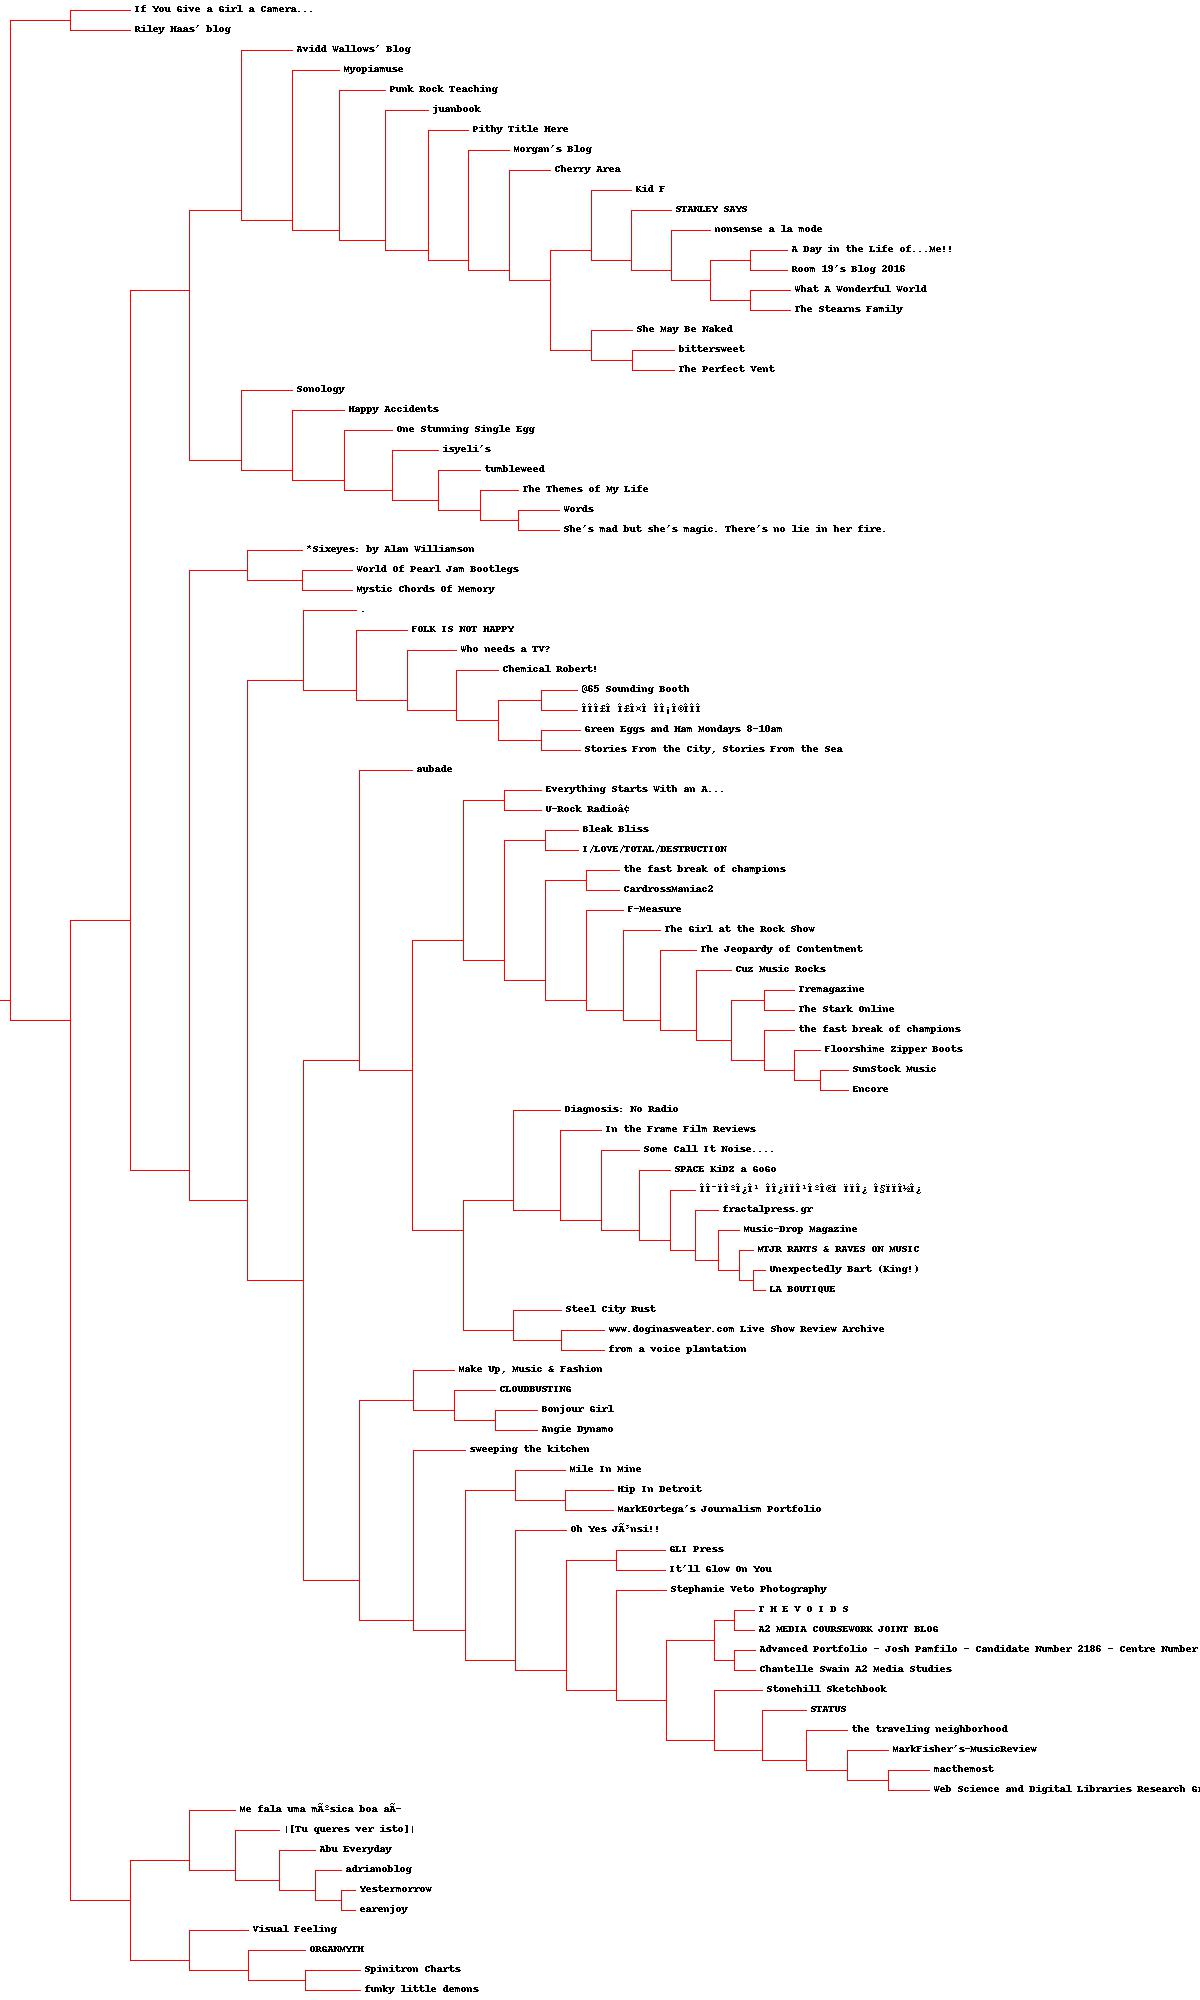
\includegraphics[width=\textwidth,height= .90\textheight]{blogMatrix.jpg}}
\end{figure}



Create an ASCII and JPEG dendrogram that clusters (i.e., HAC)
the most similar blogs (see slides 12 \& 13).  Include the JPEG in
your report and upload the ascii file to github (it will be too
unwieldy for inclusion in the report).\\

\textbf{Solution 2:}\\
 
 I used \textit{generateASCIIDendogram()} and \textit{generateJPegDendogram()} in listing 3 to create an ASCII and JPEG dendograms respectively. Listing 4 contains a snippet of the ASCII dedogram. \textit{generateASCIIDendogram()} utilizes PCI \textit{printclust()} to draw an ASCII dendogram. \textit{generateJPegDendogram()} utilizes the PCI code \textit{drawdendogram()} to draw a JPEG dendogram. Blogs JPEG dendogram is seen in Figure 1.



\end{homeworkProblem}

%----------------------------------------------------------------------------------------
% PROBLEM 3
%----------------------------------------------------------------------------------------
\begin{homeworkProblem}
\lstinputlisting[caption= K-Means Cluster Solution, language=python]{P3.py}
\lstinputlisting[caption= K-Means Cluster, language=python]{clusters.py}


Cluster the blogs using K-Means, using k=5,10,20. (see slide
18).  Print the values in each centroid, for each value of k. How
many interations were required for each value of k?\\


\textbf{Solution 3:}\\

Clustering the blogs using K-Means is achieved by using \textit{KMeans()} in listing 5. I modified \textit{scaledown()} in listing 6 in order to return the number of iterations required for each value of k. Table \ref{tab:K-means} shows the k-values and number of iterations. K5.txt, K10.txt, and K20.txt files contains K clustering counts and iterations respectively.\\


\end{homeworkProblem}


%----------------------------------------------------------------------------------------
% PROBLEM 4
%----------------------------------------------------------------------------------------
\begin{homeworkProblem}
\lstinputlisting[caption= MDS Code language=python]{P4.py}

\begin{figure}
    \caption{MDS Diagram, Required iteration = 5}
    \subfigure{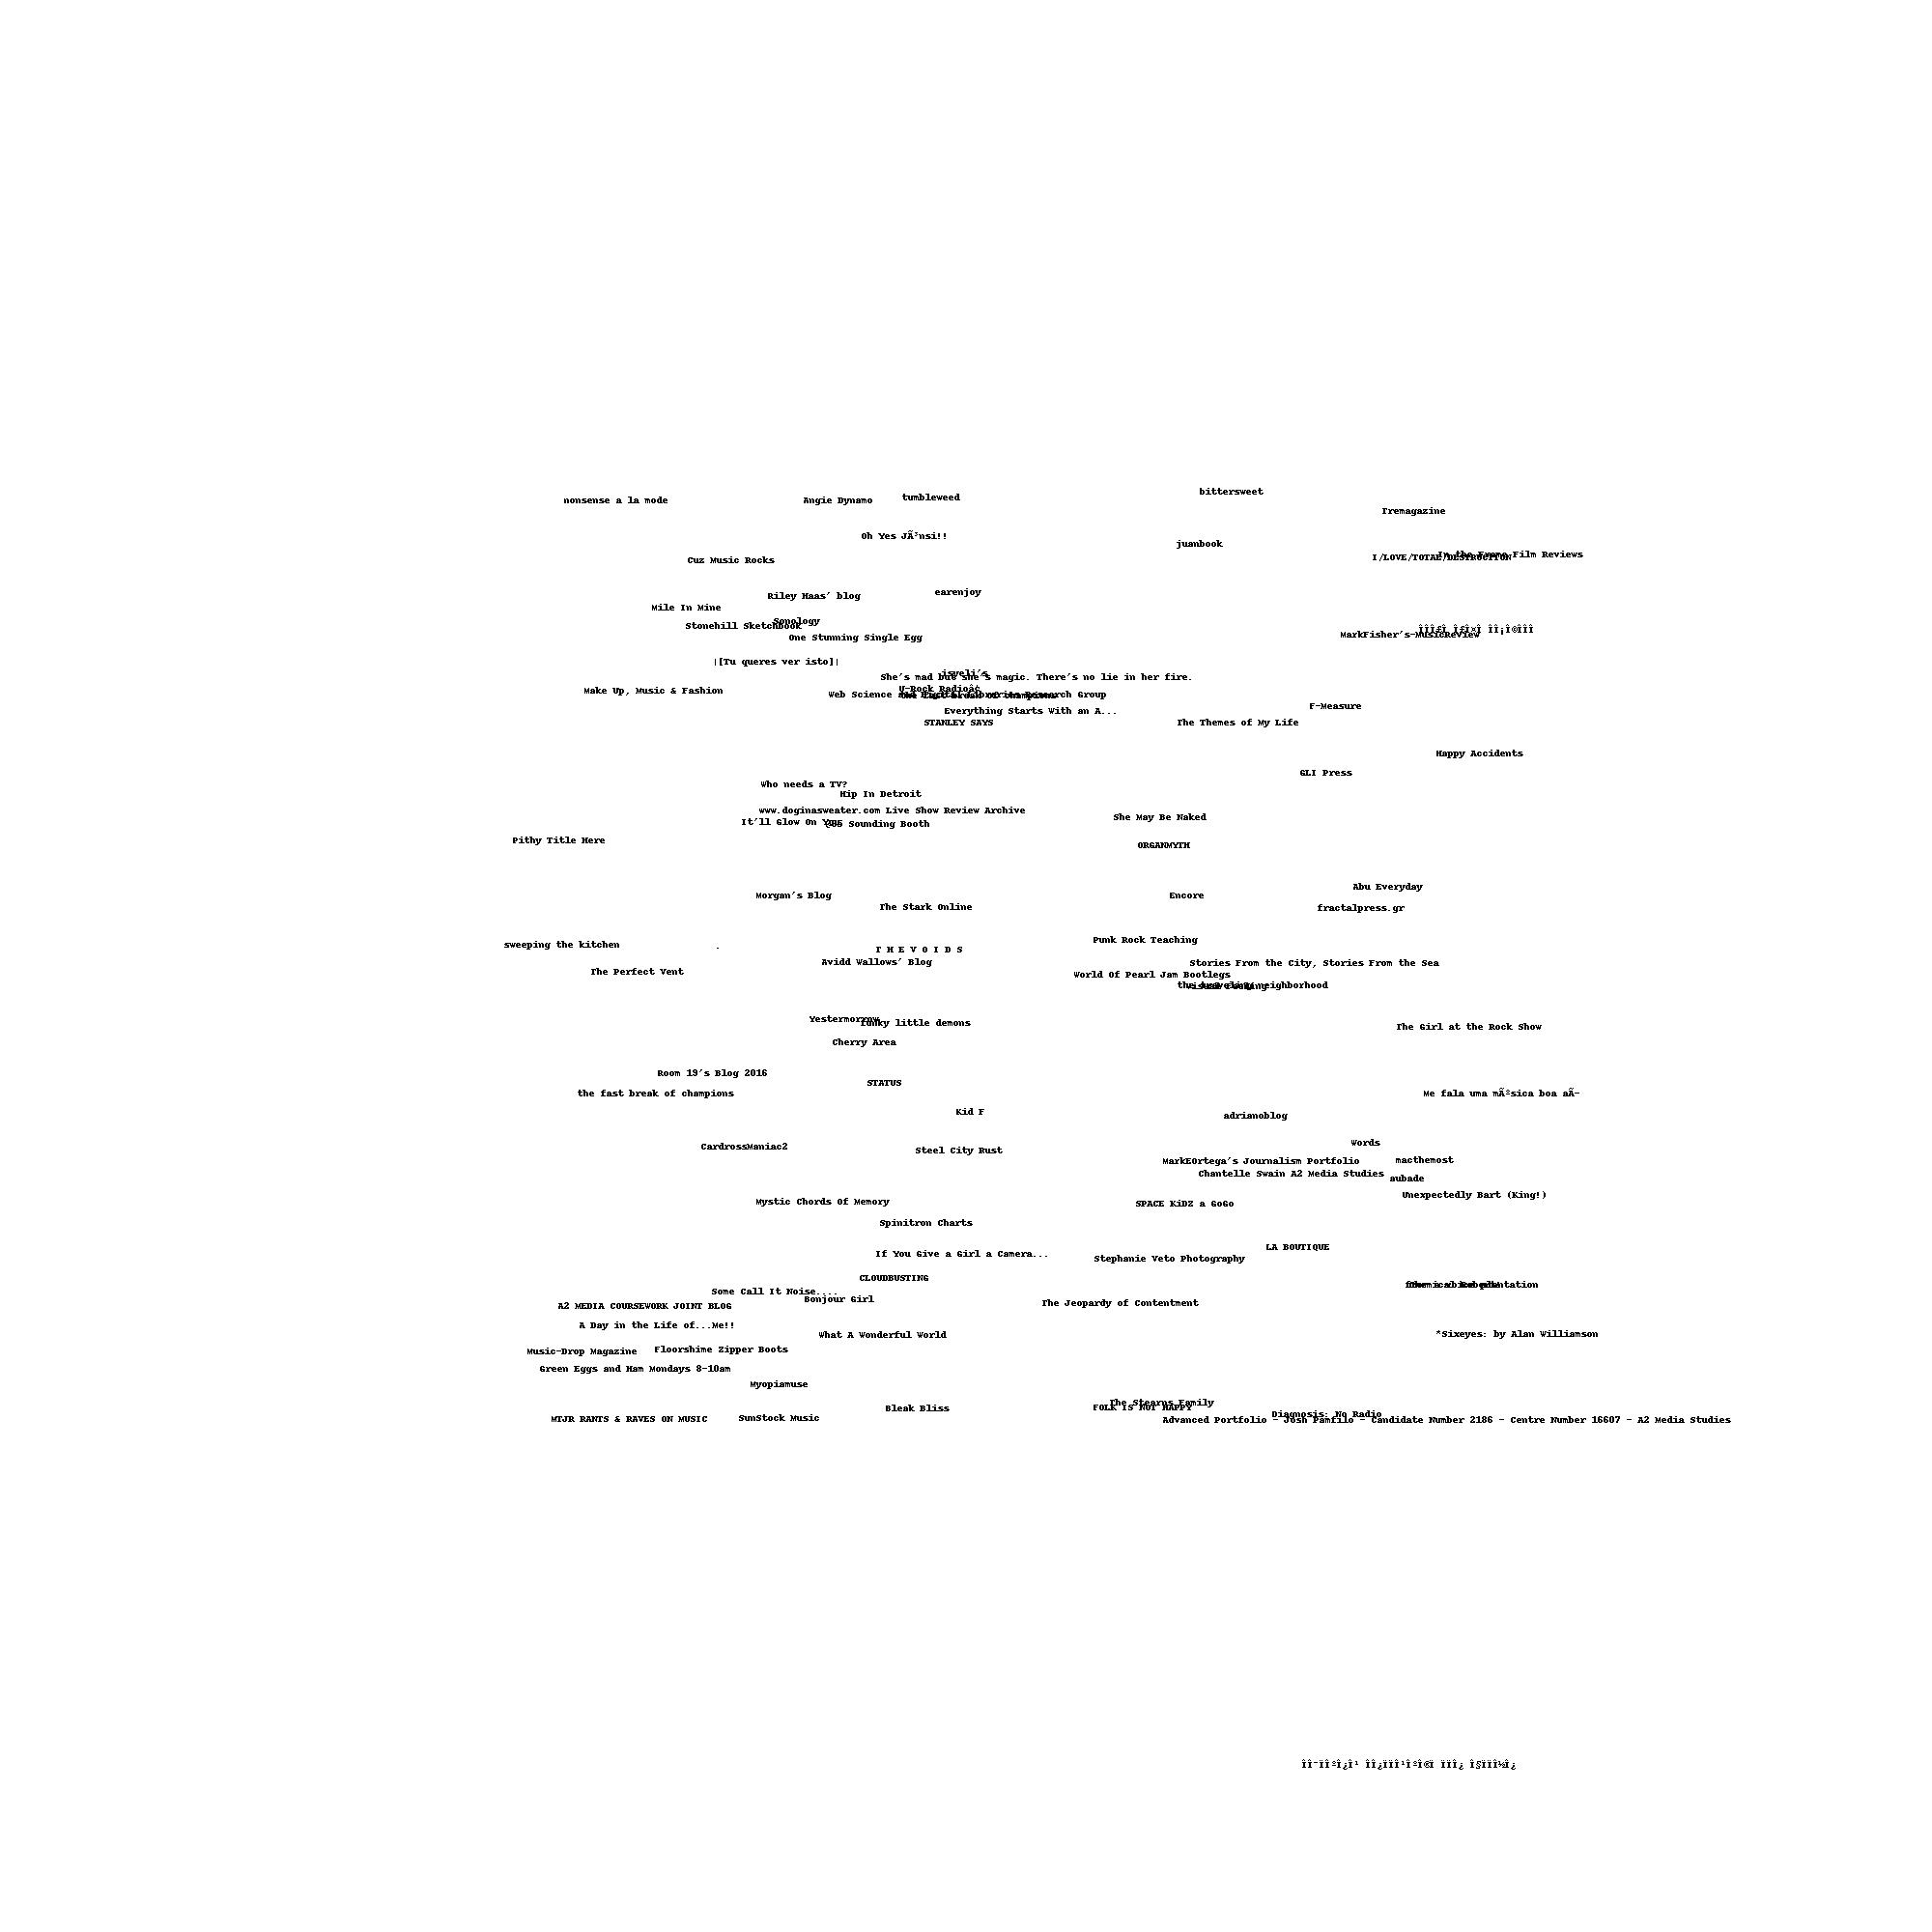
\includegraphics[width=\textwidth,height=.90\textheight]{blogmatrix.jpg}}
\end{figure}

Use MDS to create a JPEG of the blogs similar to slide 29 of the 
week 12 lecture.  How many iterations were required?\\


\textbf{Solution 4:}\\

 In order to use MDS to create a JPEG of similar blogs, I used \textit{MDS()} in listing 6. The MDS JPEG of blogs is seen in Figure 2.

 \end{homeworkProblem}




\nocite{*}\clearpage
\bibliographystyle{plain}
\bibliography{A8Ref}

































\end{document}
